\section{问题分析}


\subsection{问题一分析}

该问题本质为数据探索与特征分析问题。
核心目标是在无先验假设的条件下，
通过统计分析和可视化呈现构建流失客户群体的特征画像。
需重点关注两方面：
一是数据质量——是否存在异常值及类型不一致等影响建模的问题；
二是特征区分度——哪些变量在流失与未流失客户之间呈现显著差异。
可采用分组统计、分布对比图、相关性分析等手段进行系统探索。

\subsection{问题二分析}

该问题本质为二分类建模与模型可解释问题。
在问题一筛选的特征基础上，
构建从客户特征到流失概率的预测模型。
模型选择需兼顾精度与可解释性：
以逻辑回归为线性基准，
以随机森林和 XGBoost 为非线性对照。
评估阶段，针对类别不平衡问题采用 AUC 与 F1-score 作为主要指标；
分析阶段，引入 SHAP 方法将模型输出分解为各特征的量化贡献，
为业务决策提供数据支撑。

\subsection{问题三分析}

该问题本质为策略优化与投入产出评估问题。
基于问题二的流失概率输出，
对客户进行风险分层并将层级与客户生命周期价值（CLTV）关联，
针对不同层级客户的行为特征设计差异化挽留方案。
方案需同时权衡预期收益（减少流失所挽回的收入）与实施成本
（优惠力度与运营投入），论证收益与成本之间的经济可行性。

\subsection{数据说明}

\textbf{数据来源：}题目附件 \texttt{Telco\_customer\_churn.xlsx}。

\textbf{数据规模：}共 7043 条客户记录，33 个特征变量，
涵盖人口统计学特征（性别、年龄、家庭状况）、
账户服务信息（在网时长、合同类型、支付方式、服务开通情况）、
费用信息（月消费、总消费、生命周期价值）以及流失标签。

\textbf{数据质量：}经检查，数据整体完整无缺失值。
其中 \texttt{Total Charges} 列存在 11 条因在网时长为 0 而产生的逻辑空值，
已按业务逻辑填充为 0。剔除 \texttt{CustomerID}、\texttt{Count}、
\texttt{Country} 三个无信息量列后，剩余 30 个可用特征，全部 7043 条记录完整可用。详细的预处理步骤见第4章问题一的数据预处理节。

\textbf{目标变量分布：}流失客户 1869 人（占比 26.54\%），
未流失客户 5174 人（占比 73.46\%），
呈现一定程度的类别不平衡，后续建模需采取加权或采样策略加以应对。

\subsection{整体建模流程}

本文的整体建模流程如图 \ref{fig:flowchart} 所示。

\begin{figure}[htbp]
    \centering
    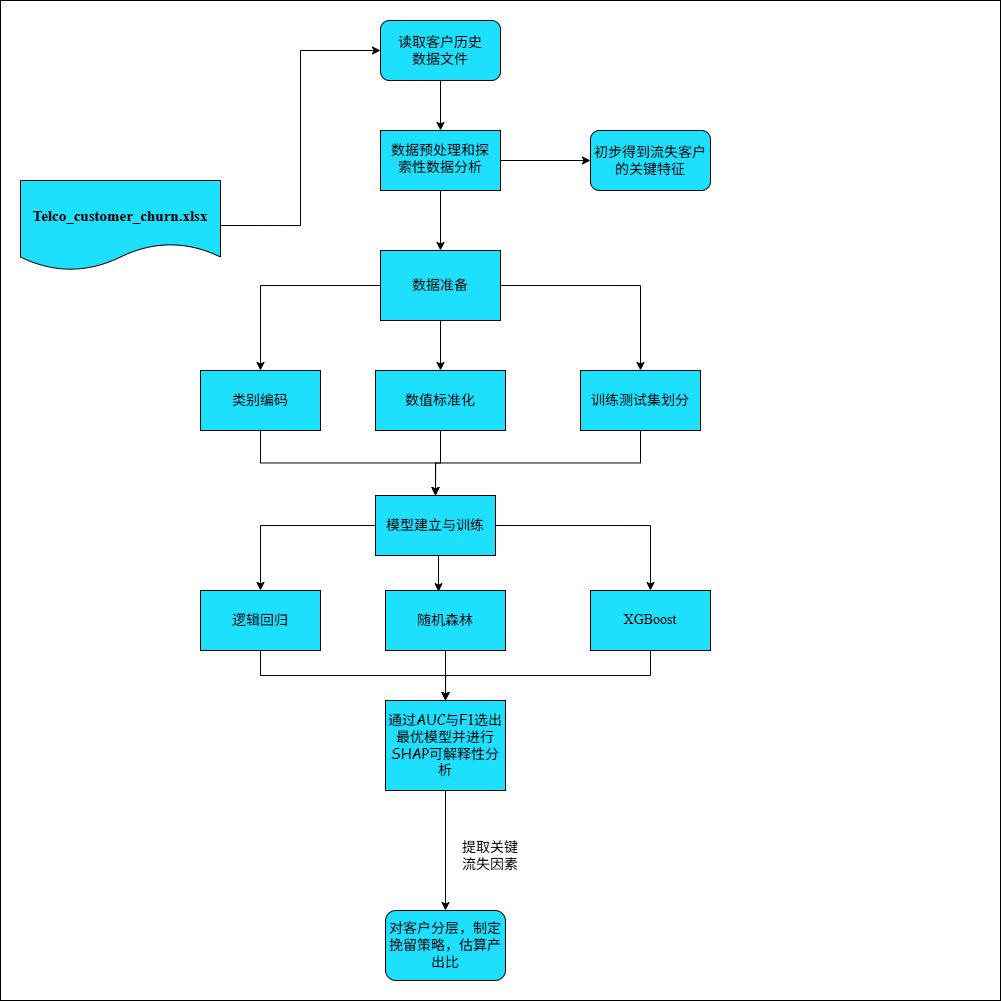
\includegraphics[width=\textwidth]{./figures/flowchart.png}
    \caption{整体建模流程}
    \label{fig:flowchart}
\end{figure}

首先进行数据预处理与探索性分析，识别数据质量问题和关键特征；
然后进行数据准备（类别编码、数值标准化、训练测试集划分），
分别训练逻辑回归、随机森林、XGBoost 三种分类模型并通过
AUC 与 F1-score 进行对比优选；
对最优模型进行 SHAP 可解释性分析，提取关键流失因素；
最后基于模型输出的流失概率进行客户分层，
制定差异化挽留策略并估算投入产出比。
